\chapter{Explicabilidad y validación clínica}
\label{cap:explicabilidad}
\begin{resumen}
	En este capítulo describimos cómo se generan y utilizan los \emph{saliency maps} para explicar las decisiones del \emph{gold standard}, detallamos la validación preliminar con un especialista y exponemos las mejoras introducidas a partir de su retroalimentación.
\end{resumen}

\section{Método de explicabilidad utilizado}
La única técnica de explicabilidad implementada en este trabajo son los \emph{saliency maps} basados en gradientes, aplicados al \emph{gold standard} exclusivamente. Esta decisión se debe a las siguientes razones:

\begin{enumerate}
	\item \textbf{Desempeño superior del \emph{gold standard}}: En el Capítulo \ref{cap:train} hemos visto que el \emph{gold standard} obtiene mejores resultados en casi todas las métricas evaluadas.
	\item \textbf{Imposibilidad de Grad-CAM en modelos transformados}: Como las redes transformadas mantienen la arquitectura con capas Conv1D, no se pueden aplicar métodos como Grad-CAM a la representación bidimensional. Además, los \emph{saliency maps} no ofrecen una explicación clara sobre imágenes, ya que tratan cada una de las filas de la entrada como datos independientes.
\end{enumerate}
\section{Resultados de explicabilidad}
Aplicando la librería de explicabilidad TSInterpret\footnote{Puede encontrarse su documentación en el siguiente \href{https://fzi-forschungszentrum-informatik.github.io/TSInterpret/}{enlace}.}, hemos explicado cinco casos del conjunto de test para cada clase que cumplen las siguientes condiciones:
\begin{itemize}
	\item El valor real de la etiqueta es solamente una condición, es decir, el valor esperado es 1.0 para una de las clases y 0.0 para el resto.
	\item La predicción es perfecta, es decir, la única etiqueta en la que el modelo clasifica el ECG es la que tiene un valor real de 1.0.
	\item La clase HYP no tiene ningún caso así, debido a que es la clase minoritaria, por lo que no hemos podido aplicar explicabilidad a esta clase.
\end{itemize}
Todas las explicaciones realizadas pueden encontrarse en la siguiente \href{https://drive.google.com/drive/folders/1EOW2RsL3Ub2UQ1NiEeRpMVd9SsnQpBkf?usp=drive_link}{carpeta}, pero en la Figura \ref{fig:explicaciones} podemos ver una imagen con la explicación de la primera derivación de un ECG de cada clase (excepto HYP).

\begin{figure}
	\centering
	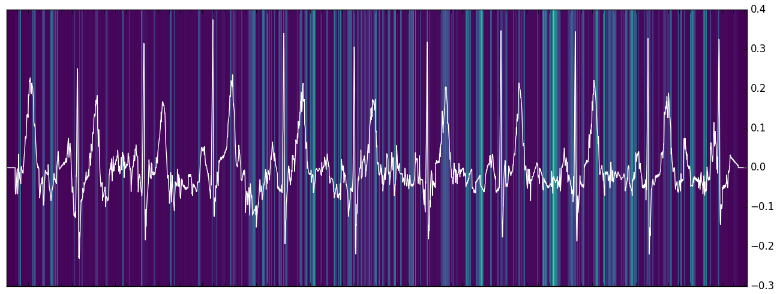
\includegraphics[width=0.9\linewidth]{Imagenes/Vectorial/explanations/NORM.png}
	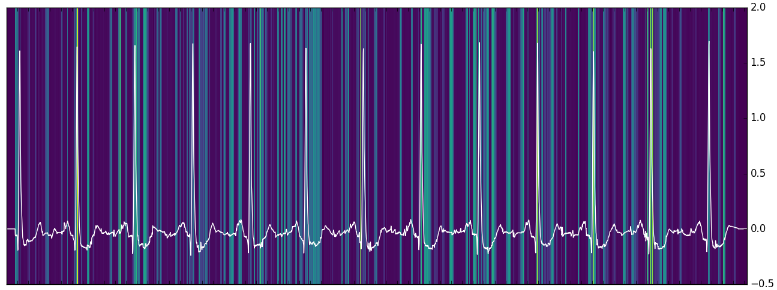
\includegraphics[width=0.9\linewidth]{Imagenes/Vectorial/explanations/MI.png}
	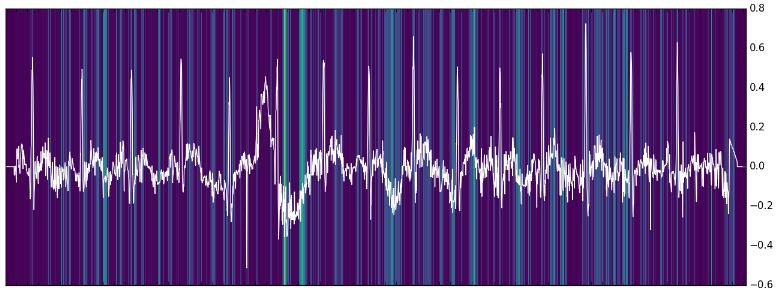
\includegraphics[width=0.9\linewidth]{Imagenes/Vectorial/explanations/STTC.png}
	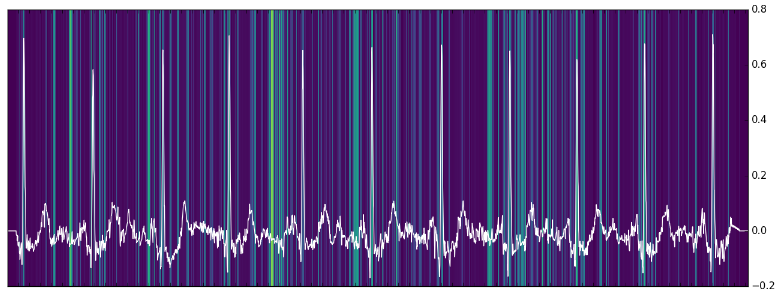
\includegraphics[width=0.9\linewidth]{Imagenes/Vectorial/explanations/CD.png}
	\caption{Explicaciones de la primera derivación de un ECG de las clases NORM, MI, STTC, CD (respectivamente)}.
	\label{fig:explicaciones}.
\end{figure}

En la Figura \ref{fig:explicacionvs} puede verse una comparación entre nuestra explicación de un infarto de miocardio y la de otro artículo, y se puede comprobar que, en efecto, los modelos se fijan en las mismas zonas (en este caso concreto, después del valle más pronunciado).

\begin{figure}
	\centering
	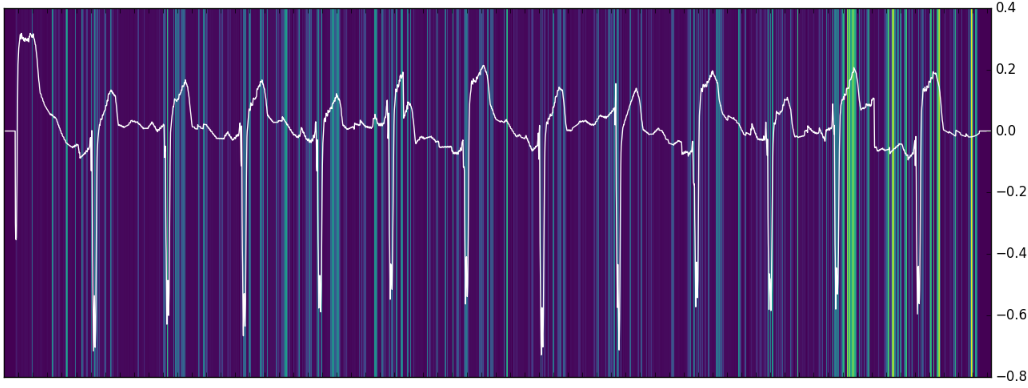
\includegraphics[width=0.9\linewidth]{Imagenes/Vectorial/Feature_7.png}
	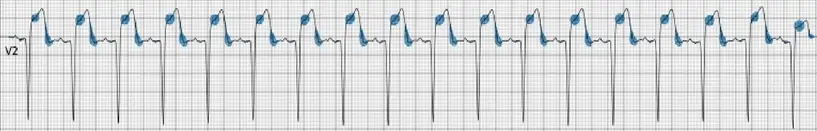
\includegraphics[width=0.9\linewidth]{Imagenes/Vectorial/V2.png}
	\caption{Explicación de un infarto de miocardio en nuestro modelo (arriba) y en un artículo de investigación (abajo). Fuente: \cite{gustafsson2022deep}.}
	\label{fig:explicacionvs}
\end{figure}

\section{Validación con los expertos médicos}
Tras hacer las explicaciones, se las mostramos a varios médicos para obtener feedback de éstas. Su opinión general es que es una herramienta con potencial de ser muy útil, y que generalmente detecta correctamente zonas donde puede verse la anomalías, pero hizo los siguientes comentarios de cara a mejorarlo:
\begin{enumerate}
	\item \textbf{Heterogeneidad de la explicación} \\
	El experto señaló que, salvo excepciones, las anomalías cardíacas se presentan en todos los latidos, no solo en algunos, por lo que es extraño que la explicación señale únicamente las anomalías en algunos latidos.
	\item \textbf{Alternativa de presentación} \\
	El experto sugirió reducir las imágenes y mostrar únicamente dos latidos del corazón, ya que esto es una forma habitual de visualizar y explicar anomalías a los médicos en formación.
	\item \textbf{Conformidad con la práctica clínica habitual} \\
	El experto señaló que la presentación que hemos hecho del ECG se separa bastante de la presentación habitual de estos. Indica que si las imágenes estuvieran estandarizadas según la práctica clínica habitual, podría ser una herramienta muy útil para la enseñanza, pero que en su estado actual podría llevar a confusión a los alumnos.
\end{enumerate}

En general el experto tiene la sensación de que esta herramienta tiene el potencial de ser algo muy útil, principalmente en el ámbito de la enseñanza, pero que necesita implementar algunos cambios antes de ser utilizada.

\section{Modificaciones a partir del feedback}
Para poder hacer la explicación homogénea en cada latido o reducir la imagen a dos latidos representativos, necesitaríamos detectar donde empieza y acaba cada latido, así como las distintas partes de la señal. Si bien es cierto que esto es algo posible, se escapa del alcance de este trabajo, por lo que no lo implementaremos.

Respecto a la representación habitual del ECG, el motivo de que esté presentado de esta forma es que hemos utilizado la propia librería de explicabilidad para dibujar las gráficas, y ésta trabaja con series temporales en general. Para abordar este problema y mejorar la presentación, hemos modificado la imagen que genera librería \emph{ecg\_plot}, de manera que también pueda plasmar los colores relativos a la explicación por encima. En la Figura \ref{fig:explicacion_modificada} podemos ver una explicación mejorada para cada clase (excepto HYP).

\begin{figure}
	\centering
	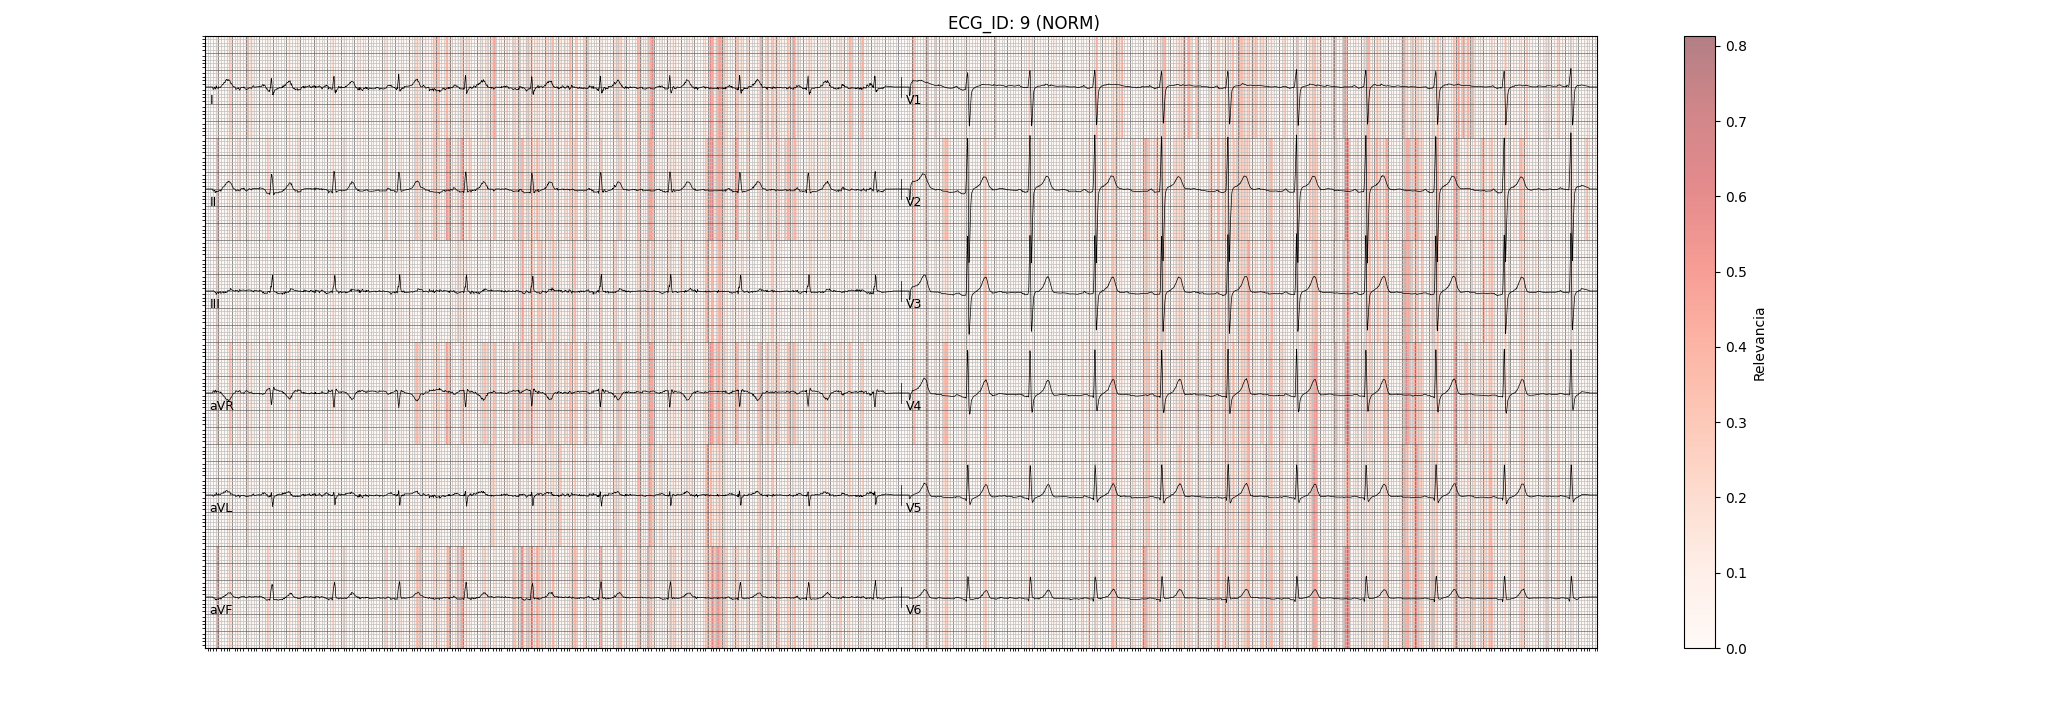
\includegraphics[width=0.9\textwidth]{Imagenes/Vectorial/better_explanations/NORM.png}
	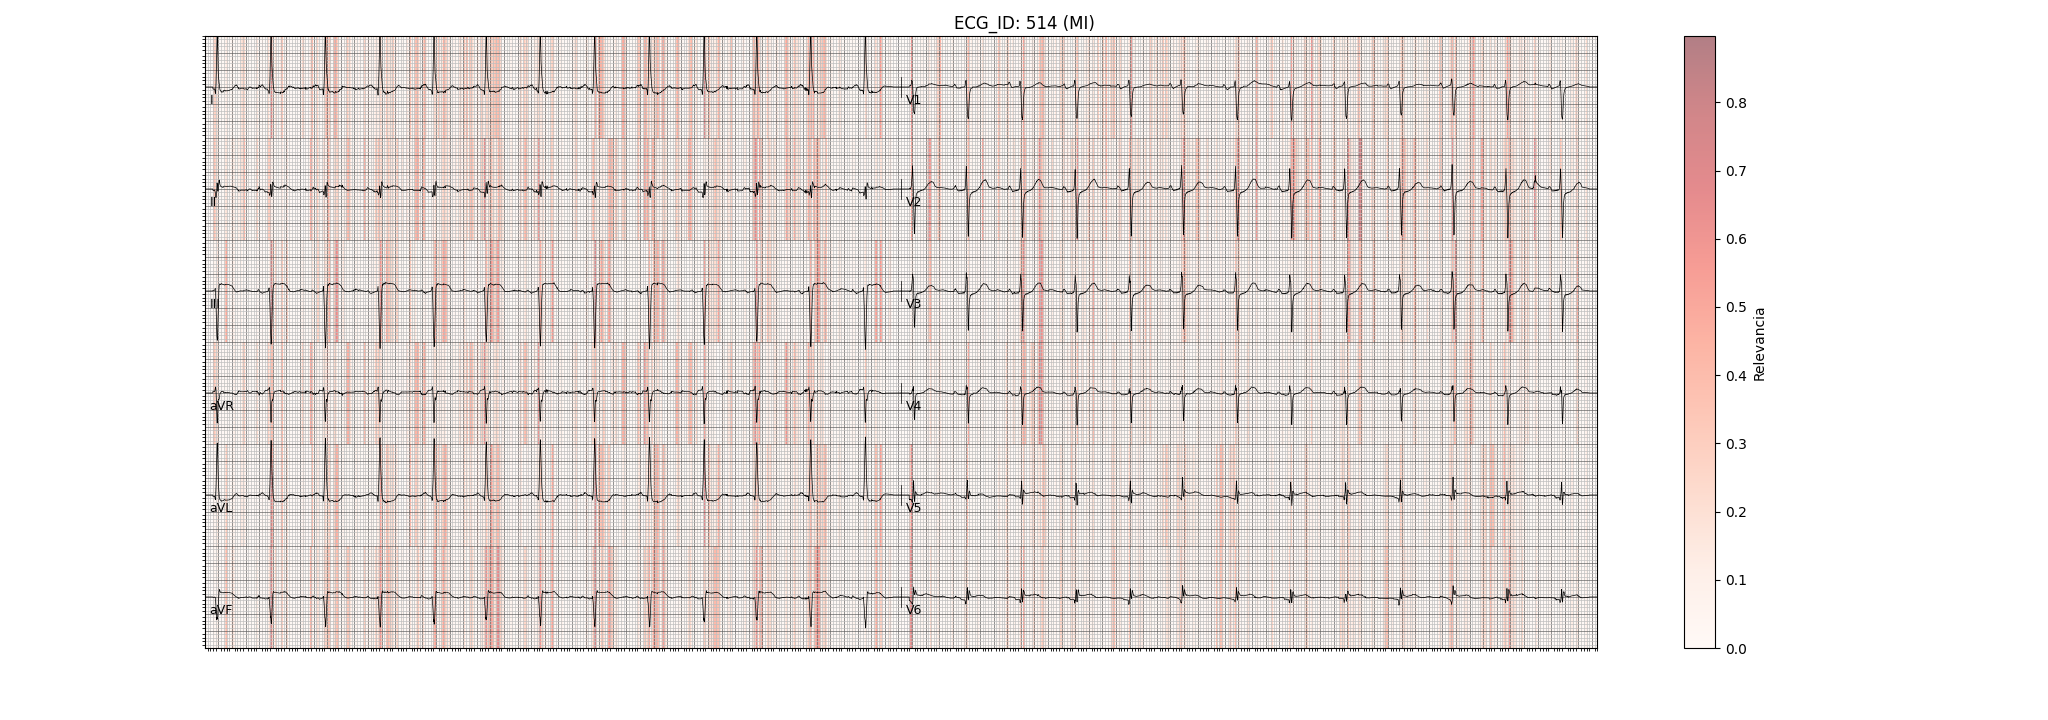
\includegraphics[width=0.9\textwidth]{Imagenes/Vectorial/better_explanations/MI.png}
	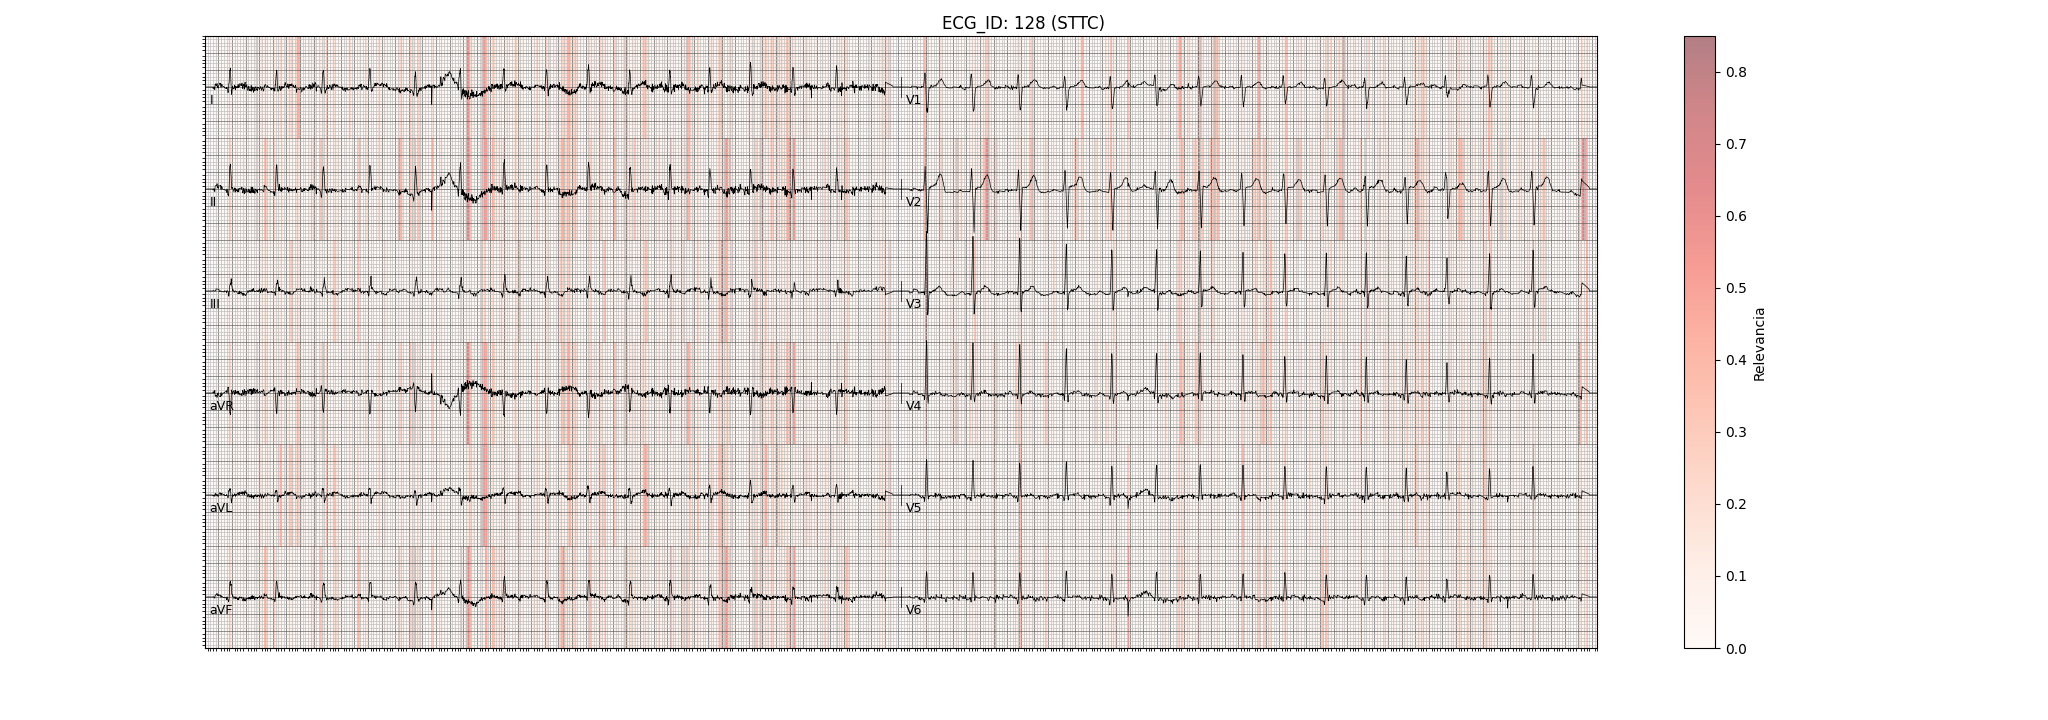
\includegraphics[width=0.9\textwidth]{Imagenes/Vectorial/better_explanations/STTC.png}
	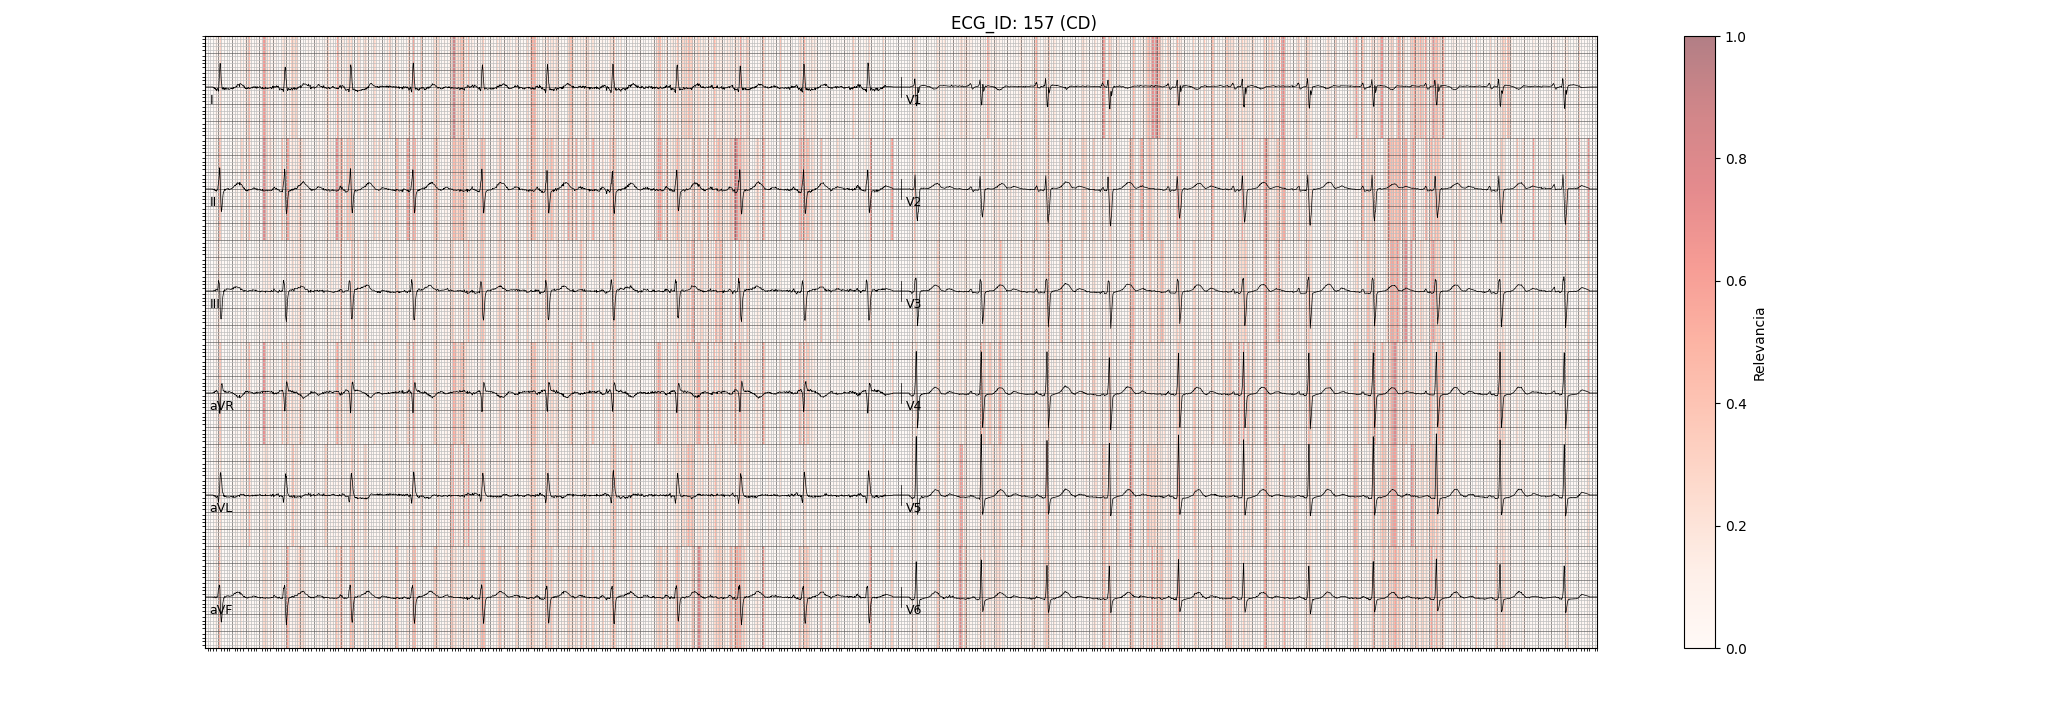
\includegraphics[width=0.9\textwidth]{Imagenes/Vectorial/better_explanations/CD.png}
	\caption{Explicación de un ECG de cada clase (excepto HYP) pintada sobre la librería \emph{ecg\_plot}}.
	\label{fig:explicacion_modificada}
\end{figure}